\chapter{Einleitung}

\section{Motivation}
Um im Unterricht Schülern und Studenten dass Programmieren und Konstruieren von Robotern zu erläutern, ist Lego Mindstorms mit dem programmierbaren Baustein NXT eine gute Wahl. Das Ziel dieser Arbeit ist es das programmieren von Lego Mindstorms Robotern zu vereinfachen und gleichzeitig die Grenzen die duch den Baustein NXT gesetzt sind zu sprengen. Wir wollen die Möglichkeiten der Programmierung des NXT eins zu eins mit dem Minicomputer Raspberry PI abbilden. Damit ist es uns möglich eine einfachere Programmierschnittstelle anzubieten und zusätzlich die vielen Möglichkeiten des Raspberry PIs für Schüler zugänglich machen. 

Wir sehen den Raspberry PI als ein dem NXT überlegenes Steuerungsmodul, da auf dem Raspberry ein vollständiges Ubuntu Linux Betriebssystem läuft. Eine Überlegung der Autoren hierbei war es auf dem Ubuntu einen Webserver laufen zu lassen und dem Roboter über diesen aus der Ferne zu steuern.
Weiterhin soll es in dieser Arbeit ermöglicht werden, weitere Sensoren an den Raspberry PI anschließen zu können. Zwar gibt es für Lego Mindstorms eine Liste von Sensoren, wie z.B einen Lichtsensor, Tastsensor und Ultraschallsensor, dieses Set an Sensoren ist allerdings eingeschränkt.

Das Bereitstellen eines programmierbaren Roboters für jeden Schüler kann schnell teuer werden. Wir sehen die Verwendung eines Raspberry PI auch deshalb als Vorteil, weil ein Raspberry B+ mit 39,90 Eur den NXT mit 9841 mit 148,99 Eur preislich schlägt. \footnote{Preisvergleich des Raspberry PI 2 B+ und NXT 9841 auf www.amazon.de}

\chapter{Grundlagen}
\section{Raspberry PI}
\label{Grundlagen:RaspberryPI}
%\index{Auszeichnungen!im Text}

Raspberry PI ist ein günstiger Computer in Kreditkartengröße, welches viele Schnittstellen bietet, wie z.B HDMI, USB, Audio, GPIOs und Ethernet.
Was den Raspberry PI so beliebt macht um eigene Systeme zu bauen, ist dass auf ihm ein vollständiges Linux Betriebssystem läuft. Dies führt dazu, dass nahezu alles was auf einem Desktoprechner läuft auch auf einem Raspberry PI ausführbar ist.

\begin{figure}[h]
  \centering
  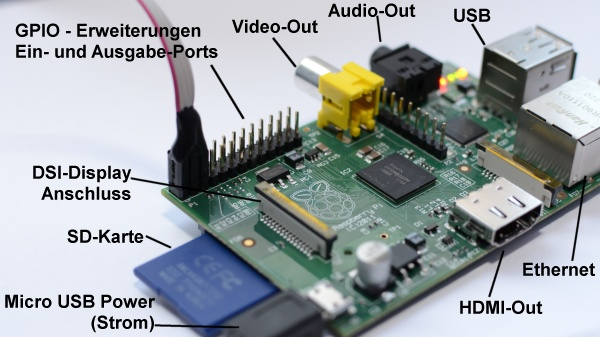
\includegraphics[width=15cm]{raspberrypi}
  \caption{Ein RaspberryPI 2 mit Beschrifteten Schnittstellen. Quelle: http://www.portunity.de/blog/2013/februar/raspberry-pi-warum-ist-der-mini-computer-bei-unseren-mitarbeitern-so-beliebt.html}
  \label{Kap1:RaspberryPI}
\end{figure}

\section{NXT}
\label{Grundlagen:NXT}
%\index{Auszeichnungen!im Text}

Lego Mindstorms NXT ist ein Steuerungscomputer der Produktserie Lego Mindstorms



\subsection{Anführungszeichen}

Deutsche Anführungszeichen gehen so: "`dieser Text steht in \glq Anführungszeichen\grq; alles klar?"'.


\subsection{Abkürzungen}
\index{Abkürzungen}
\index{Abbreviation|see{Abkürzungen}}

Eine \ac{ABK} wird bei der ersten Verwendung ausgeschrieben\footnote{Ausschreiben bedeutet, dass man nicht die Abkürzung sondern die lange Form verwendet.}. Danach nicht mehr: \ac{ABK}. Man kann allerdings die Langform\footnote{\blindtext} explizit anfordern: \acl{ABK} oder die Kurzform \acs{ABK} oder auch noch einmal die Definition: \acf{ABK}.

Mehr dazu findet sich im Kapitel~\ref{Einleitung:Textauszeichnungen} auf Seite~\pageref{Einleitung:Textauszeichnungen}.


\subsubsection{Noch ein Unterabschnitt}

\paragraph{Eine Absatzüberschrift}
\blindtext[1]


\subsection{Literaturarbeit}

Wichtig ist das korrekte Zitieren von Quellen, wie es auch von \cite{Kornmeier2011} dargelegt wird. Interessant ist in diesem Zusammenhang auch der Artikel von \cite{Vixie2007}. Häufig werden die Zitate auch in Klammern gesetzt, wie bei \citep{Kornmeier2011}.

\blindtext[4]